% include your own content here directly or with more `input`s

\newcommand{\PZprime}{\ensuremath{{\PZ}^{\prime}}\xspace}
\newcommand{\mZprime}{\ensuremath{m_{\PZprime}}\xspace}
\newcommand{\Pbifun}{\ensuremath{\Phi}\xspace}
\newcommand{\mbifun}{\ensuremath{m_{\Pbifun}}\xspace}
\newcommand{\dphij}{\ensuremath{\Delta\phi(\vec{j},\ptvecmiss)}\xspace}
\newcommand{\MHT}{\ensuremath{H_{\mathrm T}^{\text{miss}}}\xspace}
\newcommand{\met}{\ensuremath{p_{\text{T}}^{\text{miss}}}\xspace}
\newcommand{\mttwo}{\ensuremath{m_{\text{T2}}}\xspace}
\newcommand{\rinv}{\ensuremath{r_{\mathrm{inv}}}\xspace}
\newcommand{\DELPHES}{{\textsc{delphes}}\xspace}
\newcommand{\Lamdark}{\ensuremath{\Lambda_{\text{dark}}}\xspace}
\newcommand{\Ncdark}{\ensuremath{N_{c}^{\text{dark}}}\xspace}
\newcommand{\Nfdark}{\ensuremath{N_{f}^{\text{dark}}}\xspace}
\newcommand{\Pqdark}{\ensuremath{\chi}\xspace}
\newcommand{\mqdark}{\ensuremath{m_{\Pqdark}}\xspace}
\newcommand{\mdark}{\ensuremath{m_{\mathrm{dark}}}\xspace}
\newcommand{\Pmed}{\ensuremath{\mathcal{M}}\xspace}
\newcommand{\mmed}{\ensuremath{m_{\Pmed}}\xspace}
\newcommand{\Pscalar}{\ensuremath{\text{S}}\xspace}
\newcommand{\smed}{\ensuremath{\sigma_{\Pmed}}\xspace}
\newcommand{\gqdark}{\ensuremath{g_{\Pqdark}}\xspace}
\newcommand{\sbifun}{\ensuremath{y_\text{dark}}\xspace}
\newcommand{\taudark}{\ensuremath{\tau_\text{dark}}\xspace}
\newcommand{\Tdark}{\ensuremath{T_\text{dark}}\xspace}
\newcommand{\thooft}{\ensuremath{\lambda_\text{dark}}\xspace}
\newcommand{\adark}{\ensuremath{\alpha_{\mathrm{dark}}}\xspace}
\newcommand{\gdark}{\ensuremath{g_{\mathrm{dark}}}\xspace}
\newcommand{\gq}{\ensuremath{g_{\mathrm{\cPq}}}\xspace}
\newcommand{\secGEANTfour}{\mdseries{\GEANTfour}\xspace}
\newcommand{\diffu}{\texttt{CaloDiffusion}\xspace}
\newcommand{\challenge}{\textit{CaloChallenge}\xspace}
\newcommand{\glam}{\texttt{GLaM}\xspace}
\newcommand{\DEEPJET}{\textsc{DEEPJET}\xspace}

%\begin{spacing}{0.93}
\begin{spacing}{0.96}

\section{Introduction}\label{sec:intro}

This proposal addresses two important, outstanding topics in particle physics at the energy frontier:
the nature of dark matter (DM) and the computational challenge of detector simulation.
The new P5 report~\cite{P5:2023} has reaffirmed that determining the nature of DM,
as well as searching for direct evidence of new particles, are key science drivers for the field.
Further, software and computing are noted as key enablers and areas for investment.
These topics are crucial for the Large Hadron Collider (LHC) program,
including the upcoming high-luminosity upgrade (HL-LHC).

In particular, this proposal explores the hypothesis that dark matter, much like ordinary matter,
consists of composite particles bound together by a strong force, analogous to standard model (SM) quantum chromodynamics (QCD).
This is predicted by ``hidden valley'' models~\cite{Strassler:2006im}, which postulate a dark sector with a new, confining force, called ``dark QCD''.
This composite, strongly coupled dark matter is expected to have highly suppressed interactions with ordinary matter
and therefore would evade detection at direct and annihilation-based dark matter experiments~\cite{Cohen:2017pzm,Petraki:2013wwa}.
However, evidence of dark QCD may be found at colliders, illustrating the complementarity between the different prongs of the high energy physics (HEP) program.
Collider production would result in several varieties of novel phenomenological signatures,
and because these models include numerous parameters with unknown values and theoretical uncertainties, the most effective search strategy will cover a broad range of such phenomena.
This will be accomplished through unsupervised artificial intelligence (AI), which learns to distinguish known standard model (SM) processes from anomalies
without relying on a specific model of new physics.
Unsupervised AI will be employed both to select events at the trigger level and to identify new phenomena later in the analysis.

Accurate detector simulation is one of the cornerstones of HEP, crucial to design searches for new physics.
Because of the wide range of possible signal models,
as well as the potentially large backgrounds from high-cross section processes such as SM QCD multijet production,
this program will require substantial quantities of simulated events.
The current approach, modeling each simulated particle's interactions with the detector material, is too computationally intensive to deliver enough events.
In this way, the search for composite dark matter presages a challenge soon to be faced by the entire field at the HL-LHC.
With data rates increasing by a factor of 10 and event complexity growing similarly, no analysis will have a sufficient amount of simulation.
New techniques in generative AI are well suited to address this challenge, dramatically accelerating the computation of detector simulation while retaining quality.
AI-based simulation can naturally take advantage of GPUs and other coprocessors, such as those at high performance computing (HPC) centers.
Using inference as a service, these new techniques will be implemented with minimal disruption to the existing software and maximal flexibility to use coprocessors efficiently.

The PI is a recognized leader in strongly coupled dark matter and both unsupervised and generative AI.
His leadership is supplemented by broad expertise in collider searches for new physics and scientific computing.
The program proposed here will advance multiple elements of the DOE HEP mission: understanding dark matter and improving capabilities in detector simulation.
The benefits will extend to the entire field and even into the future, beyond the HL-LHC, providing physics motivation and critical techniques for future colliders.
Success will be achieved by leveraging the PI's established collaborations based at Fermilab, which provides unparalleled and highly relevant resources and knowledge.

\subsection{Dark Matter}\label{subsec:dm}

\subsubsection{Background}\label{subsec:dmbkg}

Many astronomical observations, from various independent and complementary sources,
indicate that dark matter exists, comprises the majority of matter in the universe, and does not consist of any SM particles.
These sources include:
galaxy rotation curves, most of which do not match the expectation from visible matter~\cite{Rubin:1980zd,Persic:1995ru} except for a few~\cite{vanDokkum:2018vup,PinaMancera:2021wpc}, indicating that DM is unevenly distributed;
strong gravitational lensing from galaxy cluster collisions~\cite{Clowe:2006eq} and weak gravitational lensing from large-scale structures~\cite{Chang:2017kmv};
the cosmic microwave background power spectrum~\cite{Planck:2018vyg} and the matter power spectrum of the universe~\cite{Dodelson:2011qv,Planck:2018nkj};
and discrepancies in light element abundances from big bang nucleosynthesis~\cite{Pospelov:2010hj}.

Weakly interacting massive particles (WIMPs) have been explored for decades~\cite{Jungman:1995df}, with no direct evidence yet obtained for their existence.
Numerous searches have targeted their collider signature, an excess of events with large missing transverse momentum (\ptvecmiss, with magnitude \met),
including several of the most impactful led by the PI, motivated by hadronic supersymmetry~\cite{Khachatryan:2016kdk,Sirunyan:2017cwe,Sirunyan:2019hzr,Sirunyan:2019ctn,CMS:2023xlp}.
Alternative approaches, including the direct detection of interactions between dark matter and nuclei of visible matter
and indirect detection of dark matter annihilation or decay, similarly have not detected WIMP signatures.

Dark matter has been estimated from astrophysical measurements to have an abundance similar,
on the cosmological scale, to visible matter (roughly five times greater~\cite{Ade:2015xua}).
This correspondence implies that dark matter may consist of composite particles, much like the baryons that make up the majority of visible matter~\cite{Bai:2013xga,Bodas:2024idn},
possibly arising from a similar asymmetry mechanism~\cite{Petraki:2013wwa}.
Unlike WIMPs, exploration of composite dark matter models has only just started, and many such models have not been ruled out.

\subsubsection{Objectives}\label{subsec:dmobj}

The hidden valley models that produce strongly coupled dark matter include a new $SU(\Ncdark)$ strong force that binds dark quarks (\Pqdark) into dark hadrons, creating dark showers of new particles.
Depending on the details of the particles and forces in the hidden sector,
as well as the mediator particles that facilitate weak interactions between the SM and the hidden sector,
these dark showers can produce a variety of experimental signatures.
These include: \emph{semivisible jets} (SVJs), where \met from invisible dark hadrons is aligned with visible SM hadrons~\cite{Cohen:2015toa};
\emph{emerging jets} (EMJs), with multiple displaced vertices from decays of long-lived dark hadrons~\cite{Schwaller:2015gea};
and \emph{soft unclustered energy patterns} (SUEPs), in which unsuppressed large angle emissions lead to a spherical pattern of dark hadrons~\cite{Knapen:2016hky}.
These signatures are quite distinct from the expectations from WIMP dark matter and therefore are not probed by WIMP searches.

In this proposal, we will develop and expand the existing program of dark QCD jet searches, initiated and led by the PI.
We focus on SVJs as the most subtle signature; EMJs and SUEPs present unusual but identifiable signatures in the tracking systems,
while SVJs can only be distinguished from SM QCD by careful investigation of jet substructure and event-level correlations.
We will assemble a comprehensive SVJ search strategy from several elements.
Building on the recent Snowmass effort~\cite{Albouy:2022cin}, we will continue model building to obtain a broader set of viable parameter combinations in complete hidden valley theories,
in order to understand the ranges of possible observables, catalog any degeneracies, and rule out any unphysical models.
The acceptance of conventional triggers for dark QCD models depends strongly on the production mode and associated final-state kinematics;
AI-based anomaly detection triggers promise significant increases in recorded dark QCD events.
Finally, the existing strategies for resonant and non-resonant searches will be unified, with the latest AI techniques employed,
which will allow us to produce the most impactful result more efficiently.
This program will be conducted using the LHC Run 3 dataset, which is larger and higher energy than the Run 2 dataset, offering further gains.

After the completion of the unified SVJ search, we will combine the results with the ongoing EMJ and SUEP searches.
This combination will be reinterpreted to cover new models with mixtures of all three signatures: emerging SVJs, semivisible or emerging SUEPs, and finally semivisible emerging SUEPs.
This will constitute the first multidimensional scan over the entire space of dark shower models,
and it will reveal uncovered regions of parameter space to motivate the next steps for this search program into the HL-LHC era.
Conducting this scan before the HL-LHC starts will ensure that we can optimize the trigger to maximize the acceptance for the unconstrained models.
Section~\ref{sec:darkqcd} provides more details regarding the work and new developments that will make this program a success.

\subsubsection{Team and Collaborators}\label{subsec:dmteam}

The PI started and leads the CMS Dark QCD team, which includes several Fermilab RAs (T. Klijnsma, C. Madrid, E. Smith) and scientists (D. Elvira, B. Jayatilaka, S. Mrenna).
There are also numerous university personnel via the LHC Physics Center (LPC)~\cite{LPC}, hosted at Fermilab, from various institutes:
Boston University, Massachusetts Institute of Technology, University of Colorado, University of Maryland, University of Puerto Rico, University of Rochester, and University of Tennessee.
The team additionally collaborates with international partners, associated with CERN, from ETH Zurich, Karlsruhe Institute of Technology, and University of Zurich.
In particular, we benefit from the contributions of top-tier graduate students and RAs, including several LPC Graduate Scholars, LPC Distinguished Researchers, and a Lederman Fellow.
We also stay in close contact with theorists and phenomenologists,
such as the authors of Refs.~\cite{Strassler:2006im,Cohen:2015toa,Schwaller:2015gea,Knapen:2016hky,Albouy:2022cin}, who develop and explore strongly coupled hidden sector models,
as well as Fermilab theorists who work on related areas (E. Bernreuther, G. Krnjaic).

The early career support will enable a dedicated RA to lead the new, unified Run 3 SVJ search with collaborators from this team.
This will supplement the partial effort from the RAs mentioned above and the other collaborators, many of whom focus on searches for other dark QCD phenomena (EMJs and SUEPs).
The AI-specific components of the proposal will also benefit from Fermilab's AI group and other experts, described in more detail in Section~\ref{subsec:simteam}.

\subsection{Detector Simulation}\label{subsec:sim}

\subsubsection{Background}\label{subsec:simbkg}

Full detector simulation using \GEANTfour~\cite{Agostinelli:2002hh} is highly accurate, but computationally costly:
it consumed 40\% of grid CPU usage by the major LHC experiments during Run 2~\cite{Apostolakis:2018ieg}.
This limits the number of simulated events that can be produced, directly increasing uncertainties and reducing sensitivity.
In particular, SVJ searches (Section~\ref{subsec:dm}) require large background samples to design optimal strategies
and large signal samples for thorough scans of the large signal model parameter space.
However, statistical uncertainty in simulation impacts the entire collider physics program, including measurements of the Higgs boson.

\begin{figure}[htb!]
\centering
\twofigeqh{figures/cpu_cms2022.pdf}{figures/cpu_pie_cms2022.pdf}
\caption{Left: projected CPU needs and resources for CMS in Run 3 (LHC) and Runs 4--5 (HL-LHC). Right: breakdown of CPU usage by activity during Run 4. Reproduced from Ref.~\cite{CMS-NOTE-2022-008}.
}
\label{fig:cmsoffcomp}
\end{figure}

The severity of this problem will increase dramatically for the HL-LHC, which will provide an order of magnitude more data,
with similar growth in the complexity of each event from the associated detector upgrades.
Figure~\ref{fig:cmsoffcomp} illustrates the extreme computing challenges in the HL-LHC era.
The proportion of computing used for reconstruction increases because of superlinear scaling of key algorithms with the number of collisions per event.
Reconstruction has received substantial community attention and effort to pursue algorithmic and technical improvements,
such as GPU-based implementations of tracking and pulse shape fitting already deployed by CMS in Run 3~\cite{Bocci:2020pmi}.
However, the challenges facing simulation have been relatively underserved, and dedicated, coordinated effort is needed.
The CPU time used by the full detector simulation is expected to increase by a factor of 3 or more~\cite{Pedro:2020kbk},
because the detector upgrades introduce more complex geometries and higher precision that requires more detailed physics models.

The CMS detector simulation already benefits from numerous technical optimizations and physics-preserving approximations,
which improve its CPU efficiency by a factor of 4--6 compared to the default, as demonstrated by the PI~\cite{Pedro:2019mkq}.
The PI also led the effort to integrate a modernized CPU-based simulation engine in the CMS software (CMSSW)~\cite{Pedro:2020kbk},
concluding that further gains from vectorization and other improvements are ultimately limited~\cite{Amadio:2020ink}.
He now consults on the implementation of the GPU-based simulation engine Celeritas~\cite{Tognini:2022nmd} in CMS;
this project offers promising gains in simplified examples, but its performance on the full CMS geometry and physics interactions has yet to be established.
Generative AI offers an alternative and complementary approach that has been identified as meriting further exploration in the recent DOE report~\cite{AI4SES}.

\subsubsection{Objectives}\label{subsec:simobj}

In order for a generative AI algorithm to become a broadly useful replacement for full detector simulation,
it must provide a similar level of quality while substantially increasing computational efficiency.
Numerous techniques have been attempted, as summarized in Refs.~\cite{Adelmann:2022ozp,Hashemi:2023rgo}.
Most have not reached the desired level of quality, which is the necessary prerequisite for any potential increases in computational speed to be meaningful.
The PI formed and leads the CMS Machine Learning for Simulation (ML4Sim) group, and previously convened the HEP Software Foundation Detector Simulation Working Group
and the Theoretical Calculations and Simulation topical group for the Snowmass Computational Frontier~\cite{Boyle:2022cvo,Elvira:2022wyn}.
Through these roles, he has directed the field toward an emphasis on practical usability of generative AI.

The PI was among the first to explore ``denoising'' techniques~\cite{Banerjee:2022gkg}, which learn a regression from a low-quality or ``noisy'' simulation to a high-quality or ``denoised'' final result~\cite{Pixar}.
More recently, diffusion models have come to dominate generative tasks in industry, such as the popular text-to-image generators Stable Diffusion, DALL${\cdot}$E, and Midjourney.
Diffusion models can be seen as the ultimate denoising method: they learn to smear existing simulations by successively adding small amounts of randomness,
in order to be able to reverse the process, iteratively unsmearing random inputs to produce realistic output.
The PI has demonstrated that diffusion models can achieve the necessary quality, based on public datasets~\cite{Amram:2023onf}.
We will now apply this approach to simulate particle showers in the CMS calorimeters, which are the major contributor to increasing per-event simulation time at the HL-LHC~\cite{Pedro:2020kbk}.
Both ``fully generative'' (producing showers from completely random input) and ``hybrid'' (producing showers from approximately correct input) will be explored.
We target percent-level agreement with \GEANTfour and more than a factor of 10 improvement in throughput;
the former is achievable given existing results, while further increasing the speed of diffusion is an important goal of the project.
Any remaining discrepancies between the full and AI-based simulations will be handled by high-level refinement,
another regression-based technique developed by the PI~\cite{Bein:2023ylt} that is already being commissioned by CMS for Run 3.
The readiness of the entire AI-based CMS simulation chain before the HL-LHC startup will facilitate the dark QCD scan, the Run 3 capstone, as well as all Run 4 activities.

AI algorithm inference uses a restricted set of operations, such as matrix multiplications, which can naturally be accelerated on coprocessors.
The PI is the lead developer for the Services for Optimized Network Inference on Coprocessors (SONIC) approach,
which has demonstrated seamless integration of coprocessors into experiment software frameworks, with inference speedups of multiple orders of magnitude,
for CMS, ATLAS, the Deep Underground Neutrino Experiment (DUNE), the Laser Interferometer Gravitational-Wave Observatory (LIGO), and analysis facilities~\cite{Duarte:2019fta,Krupa:2020bwg,Wang:2020fjr,Rankin:2020usv,Gunny:2021gne,Cai:2023ldc,CMS:2023not,Savard:2023wwi}.
SONIC implements inference as a service, enabling usage of remote coprocessors and batching computation across events.
Deploying generative AI for simulation via SONIC provides a path for efficient utilization of HPC resources and even new, unforeseen coprocessors.
SONIC has already been shown to work with GPUs, FPGAs, TPUs (tensor processing units), and IPUs (intelligence processing units).

The impact of AI-based simulation will be felt even beyond the HL-LHC.
P5 has recommended~\cite{P5:2023} an increase in research and development toward future colliders that can reach higher energy scales
to further our exploration of the universe, including the nature of dark matter.
In particular, the report highlights a muon collider as a path to 10\TeV parton center-of-mass energy, potentially at Fermilab.
Simulation studies are one of the first critical items to understand the feasibility and design of the muon collider and its detectors.
These simulations face an even greater challenge: the beam-induced background (BIB) from muon decays in flight presents unprecedented particle multiplicity,
to the extent that a single event currently takes 24 hours to simulate in \GEANTfour.
A combination of the Celeritas GPU-based classical simulation engine and AI-based simulation using diffusion models will be necessary to handle the BIB at scale.
Delivering this application by the end of the grant period will help ensure the success of the next generation of collider experiments.

\subsubsection{Team and Collaborators}\label{subsec:simteam}

Through past work in detector simulation, the PI has established collaborations with experts in this topic at Fermilab, CERN, and the HEP Software Foundation.
In particular, Fermilab hosts one of the largest \GEANTfour groups (P. Canal, D. Elvira, S. Y. Jun, G. Lima), with whom the PI works closely;
they collaborate with Oak Ridge and Argonne national laboratories on the Celeritas project.
Fermilab also has a diverse but tight-knit group of AI experts working on collider (O. Amram, Y. Feng, L. Gray, B. Hawks, C. Herwig, T. Klijnsma, J. Ngadiuba, N. Tran),
neutrino (G. Perdue, M. Wang, T. Yang), astrophysics (A. Ciprijanovic, R. Nevin, B. Nord, M. Voetberg), and computing (M. Acosta Flechas, B. Holzman) applications.
The PI works closely with the CMS experiment software framework developers (C. Jones, D. Dagenhart, M. Kortelainen, K. Knoepfel, E. Sexton-Kennedy).
The initial investigation of ML denoising was conducted with Fermilab interns (students from University of Chicago, University of Maryland, and Lafayette College) and students and postdocs from University of Puerto Rico.
As leader of the CMS ML4Sim group, the PI collaborates closely with international colleagues from institutes such as DESY, University of Hamburg, and National Taiwan University.
The PI developed inference as a service for experiment software frameworks as part of the Fast Machine Learning Lab~\cite{FML},
a collective that includes Fermilab researchers (above)
and others from CERN, Massachusetts Institute of Technology, Purdue University, University of California San Diego, University of Colorado Boulder, University of Illinois Urbana-Champaign, and University of Washington.
The Fast ML Lab has strong ties to industry, including Nvidia and Graphcore, and the PI in particular has extensive experience working with industry engineers.
This diverse group, which the PI can most effectively access as a fellow lab scientist,
provides unparalleled knowledge and experience to support the proposal's technical and ML-related goals.
The PI's position and connections at Fermilab, therefore, act as multipliers for the DOE's early career investment, strengthening the results and impact of the proposal.

The PI and the new RA will be assisted in this project by AI associates (post-baccalaureate researchers with AI-relevant degrees and experience), supported by the early career funds.
We expect to employ two AI associates, one during budget years (BYs) 2--3 to help develop the diffusion algorithm is being developed, and a second during BYs 4--5, to implement inference as a service for simulation and utilize HPCs.
\section{Strongly Coupled Dark Matter}\label{sec:darkqcd}

\subsection{Models}\label{subsec:models}

Dark QCD models include numerous parameters, with current searches focusing on those most immediately observable:
the mediator mass \mZprime or \mbifun, the dark hadron mass scale \mdark, and the invisible fraction \rinv.
The latter is the most novel parameter of the model, corresponding to the fraction of dark hadrons that are stable and invisible (DM candidates).
However, it is an effective parameter, summarizing the impacts of various accidental symmetries and conserved quantum numbers.
Many other dark sector parameters can impact the collider final state, including the cutoff scale \Lamdark, the dark quark mass \mqdark, the number of dark colors \Ncdark, and the number of dark flavors \Nfdark.
The details of the mediator connecting the SM and dark sector, such as its couplings, can affect the decays of unstable dark hadrons.
In addition, because low-energy QCD bound state formation via showering and hadronization is non-perturbative, it must be simulated using phenomenological models,
with parameters that are tuned to measurements of SM QCD.

The models currently investigated in CMS searches are based on Refs.~\cite{Cohen:2015toa,Cohen:2017pzm}, along with contributions from the PI
regarding the relationship between \mdark and \Lamdark, as well as the modeling of \rinv~\cite{Albouy:2022cin}.
These models choose $\Ncdark=2$ and $\Nfdark=2$, which leads to similarities in baryon and meson states that may not be modeled correctly,
given the lack of a confining $SU(2)$ force in the SM.
Here, we propose a more comprehensive assessment of the interplay between \Nfdark, \Lamdark, \mdark, and \mqdark (among other parameters),
focusing on the $\Ncdark=3$ case, for which lessons from the SM, especially from lattice QCD, can be more easily reused.
This will complete the original vision of the Snowmass effort, Ref.~\cite{Albouy:2022cin},
to deliver a complete set of benchmarks covering the entire range of \rinv values from 0 to 1,
reflecting new understanding about degeneracies in the model space and any nontrivial correlations between \rinv and observables such as jet substructure.
This new set of benchmarks can guide the Run 3 search strategy to ensure the entire known phase space is covered
and can serve to unify the efforts of different experimental collaborations, which currently study different models.

\subsection{Strategy}\label{subsec:strategy}

\begin{figure}[htb!]
\centering
\twofigeqh{figures/comp_limit_dijet_new_svj_monojet_2d.pdf}{{figures/comp_gq_dijet_orig_svj_monojet_rinv0.3}.pdf}
\caption{Excluded regions of the \mZprime-\rinv plane (left) and limits on \gq (right) from the SVJ search, dijet search, and monojet search.
}
\label{fig:svjexcl}
\end{figure}

The PI led the first search for semivisible jets, published in Ref.~\cite{CMS:2021dzg}, which targeted $s$-channel production via a massive \PZprime mediator.
This is the first dedicated analysis of collider events with jets aligned with missing transverse momentum,
a signature that usually arises in the SM via undermeasurement of a jet from a QCD multijet process.
This work built on the PI's previous leadership of searches for strongly-produced supersymmetric particles in hadronic final states~\cite{Khachatryan:2016kdk,Sirunyan:2017cwe,Sirunyan:2019hzr,Sirunyan:2019ctn,CMS:2023xlp}.
The search also introduced the dual strategy of providing both model-independent and model-dependent results,
with the latter utilizing a boosted decision tree (BDT) trained to identify SVJs from specific signal models using high-level variables focusing on jet substructure.
Figure~\ref{fig:svjexcl} compares the mass and coupling exclusions from this search to the dijet resonance search, which targets the complementary process $\PZprime \to \cPq\cPaq$,
and the monojet search, which targets a signature of simplified DM models, \ptmiss in association with an initial-state radiation (ISR) jet.
Even the simple cut-based model-independent strategy offers a noticeable improvement over other searches in the area around $\rinv=0.3$, where the acceptance is maximized.

% centered, fixed-width column type
\newcolumntype{C}[1]{w{c}{#1}}
\newlength\searchlen
\setlength\searchlen{1cm}
\newlength\searchlena
\setlength\searchlena{2\searchlen}
\newlength\searchlenb
\setlength\searchlenb{3\searchlen}
\newlength\searchlenc
\setlength\searchlenc{6\searchlen}

\begin{table}[!hbtp]
\vspace{\myfigurespacing}
\centering
\begin{tabular}{c|*{6}{C{\searchlen}}}
\hline
\multirow{2}{*}{Mediator} & \multicolumn{6}{C{\searchlenc}}{Mass range} \\
& \multicolumn{2}{C{\searchlena}}{Low} & \multicolumn{2}{C{\searchlena}}{Medium} & \multicolumn{2}{C{\searchlena}}{High} \\
\hline
\PZprime & \multicolumn{2}{C{\searchlena}}{\cellcolor{yellow!50}\makecell{standard\\(boosted)}} & \multicolumn{2}{C{\searchlena}}{\cellcolor{magenta!50}\makecell{scouting\\\vphantom{(boosted)}}} & \multicolumn{2}{C{\searchlena}}{\cellcolor{orange!50}\makecell{standard\\\vphantom{(boosted)}}} \\
\hline
\Pbifun & \multicolumn{3}{C{\searchlenb}}{\cellcolor{orange!50}\makecell{standard\\\vphantom{(boosted)}}} & \multicolumn{3}{C{\searchlenb}}{\cellcolor{magenta!50}\makecell{scouting\\\vphantom{(boosted)}}} \\
\hline
\end{tabular}
\vspace{\myfigureskip}
\caption{A summary of the conventional trigger options to target different mediators and mass ranges for SVJ production.}
\label{tab:conventional}
\end{table}

Subsequently, the PI has developed several more searches, now nearing completion, that use the LHC Run 2 dataset to target different mass ranges and production modes:
low-mass \PZprime, intermediate-mass \PZprime, and nonresonant $t$-channel production through a bifundamental scalar mediator \Pbifun,
which has Yukawa couplings \sbifun between SM quarks and dark quarks~\cite{Cohen:2017pzm}.
Each search requires a different trigger strategy, summarized in Table~\ref{tab:conventional}.
These include conventional triggers based on jet \pt, \HT (the scalar sum of jet \pt), and \ptmiss;
triggering on ISR jet \pt in a boosted topology;
and the use of data scouting, in which a lower threshold in the \HT trigger is enabled by storing only partial event information~\cite{Mukherjee:2019anz}.

Here, we propose a new, unified trigger strategy in Run 3, made possible by the introduction of anomaly detection triggers that exploit unsupervised AI.
Two complementary algorithms are available: CICADA~\cite{CMS-DP-2023-086}, which looks for anomalous calorimeter clusters, and AXOL1TL~\cite{CMS-DP-2023-079}, which looks for global anomalies.
These algorithms are developed by the PI's Fermilab, CERN, and LPC colleagues, and the PI has been involved with validating and improving the performance of these triggers on dark QCD models;
the latest results are shown in Fig.~\ref{fig:svjanomaly}.
The anomaly triggers promise substantial improvements in the signal trigger efficiency, especially for lower-mass \PZprime mediators and nonresonant production,
which will facilitate sensitivity to more models and smaller couplings.

\begin{figure}[htb!]
\centering
\twofigeqh{figures/axol1tl_score_schan.pdf}{figures/axol1tl_score_tchan2.pdf}
\caption{Score distributions from anomaly triggers on SVJ processes. (PLACEHOLDER)}
\label{fig:svjanomaly}
\end{figure}

We will further unify the offline analysis strategy to cover all production modes.
Currently, no search targets resonant production of \Pbifun, which can occur singly in association with a low-\pt SVJ, or in a pair;
the resonant production modes are more prominent for low mediator mass and small \sbifun.
For all resonant cases, we will use optimal mass variables designed by semi-supervised, interpretable AI, which the PI has demonstrated to be more precise than the standard transverse mass and similar variables~\cite{Pedro:2023sdp}.
In the nonresonant case, the search must be performed in the tail of the \ptmiss distribution;
however, using the same dataset and sharing most event selection criteria with the resonant searches will significantly streamline the effort.
Even a common background estimation technique will be employed, utilizing the new ``closure loss'' developed by the PI and his colleagues,
which optimizes the output of a neural network to be able to perform an ``ABCD'' background estimation using three control regions in observed data~\cite{Crossman:2023aps}.

The most important element will be the identification or ``tagging'' of SVJs, which is the only way to reduce the large SM backgrounds beyond basic event-level kinematic selections.
From the original BDT, the team has progressed to more sophisticated approaches:
a supervised (model-dependent) tagger using particle-level inputs, based on the ParticleNet graph neural network architecture~\cite{Qu:2019gqs};
and an unsupervised (model-independent) autoencoder (AE) using jet substructure variables.
The current performance of these algorithms is shown in Fig.~\ref{fig:svjtaggers}, quantified by integrating the receiver-operator characteristic (ROC) curve to produce the area under the curve (AUC).
A comparable ParticleNet-based supervised tagger for EMJs has AUC scores of 0.97--0.99, indicating that it is markedly more difficult to distinguish SVJs from QCD jets.

\begin{figure}[htb!]
\centering
\twofigeqh{figures/rocScoreSigP2DQCD_rinv.pdf}{figures/WNAE_performance_from_SVJ_t_channel_status_update_2024_02_06-2.pdf}
\caption{The AUC performance of the latest SVJ taggers: supervised ParticleNet (left) and unsupervised Wasserstein normalized autoencoder (right).
A score of 1.0 would indicate perfect discrimination between signal and background jets.}
\label{fig:svjtaggers}
\end{figure}

The AE only learns to reconstruct common SM background processes and therefore discriminates against other processes by failing to reconstruct their kinematic features.
The PI was among the first to demonstrate the autoencoders could discriminate between SM QCD jets and SVJs, even surpassing a supervised tagger when applied to a signal model not used during training~\cite{Canelli:2021aps}.
To achieve discrimination against \ttbar jets, the normalized autoencoder (NAE) formalism~\cite{Dillon:2022mkq} was adopted in order to minimize complexity bias.
The team developed a completely novel method to stabilize the training by directly minimizing the Wasserstein or earth mover's distance
between samples drawn from the input data and from the latent representation of the autoencoder, resulting in the WNAE~\cite{Eble:2024tpr}.
This approach is also now being applied to improve the performance of the AXOL1TL anomaly trigger.

For the Run 3 SVJ search, we will develop a new tagger combining the best features of both approaches:
a graph-based autoencoder (GAE), using the Lund plane representation following Ref.~\cite{Dreyer:2020brq} and trained with the WNAE approach.
Early attempts indicate the WNGAE could approach the performance level of the supervised tagger, while remaining naturally model-independent.
While these taggers are initially trained using simulated events,
the semi-supervised universal domain adaptation technique developed by the PI and his collaborators~\cite{Ciprijanovic:2023hrw}
will be employed to ensure similar performance in data by learning only physically invariant features.

\subsection{Dark QCD Scan}\label{subsec:darkscan}

While this proposal focuses on SVJs, there are other dark QCD phenomena.
EMJs may form if the unstable dark hadrons have a lifetime \taudark, leading to multiple displaced vertices within a single jet.
SUEPs occur when there is a large 't Hooft coupling strength $\thooft = \gdark^2 \Ncdark$,
resulting in a high multiplicity of low-momentum tracks from unsuppressed large angle emissions, rather than collimated jets.
The CMS Dark QCD team has recently released new results for both signatures in Refs.~\cite{CMS:2023vpb,CMS:2024emj},
following the first CMS EMJ search with a small dataset~\cite{Sirunyan:2018njd}.
Conducting separate searches for each phenomenon is important to understand the kinematic phase space and behavior associated with these new models.

\begin{figure}[htb!]
\centering
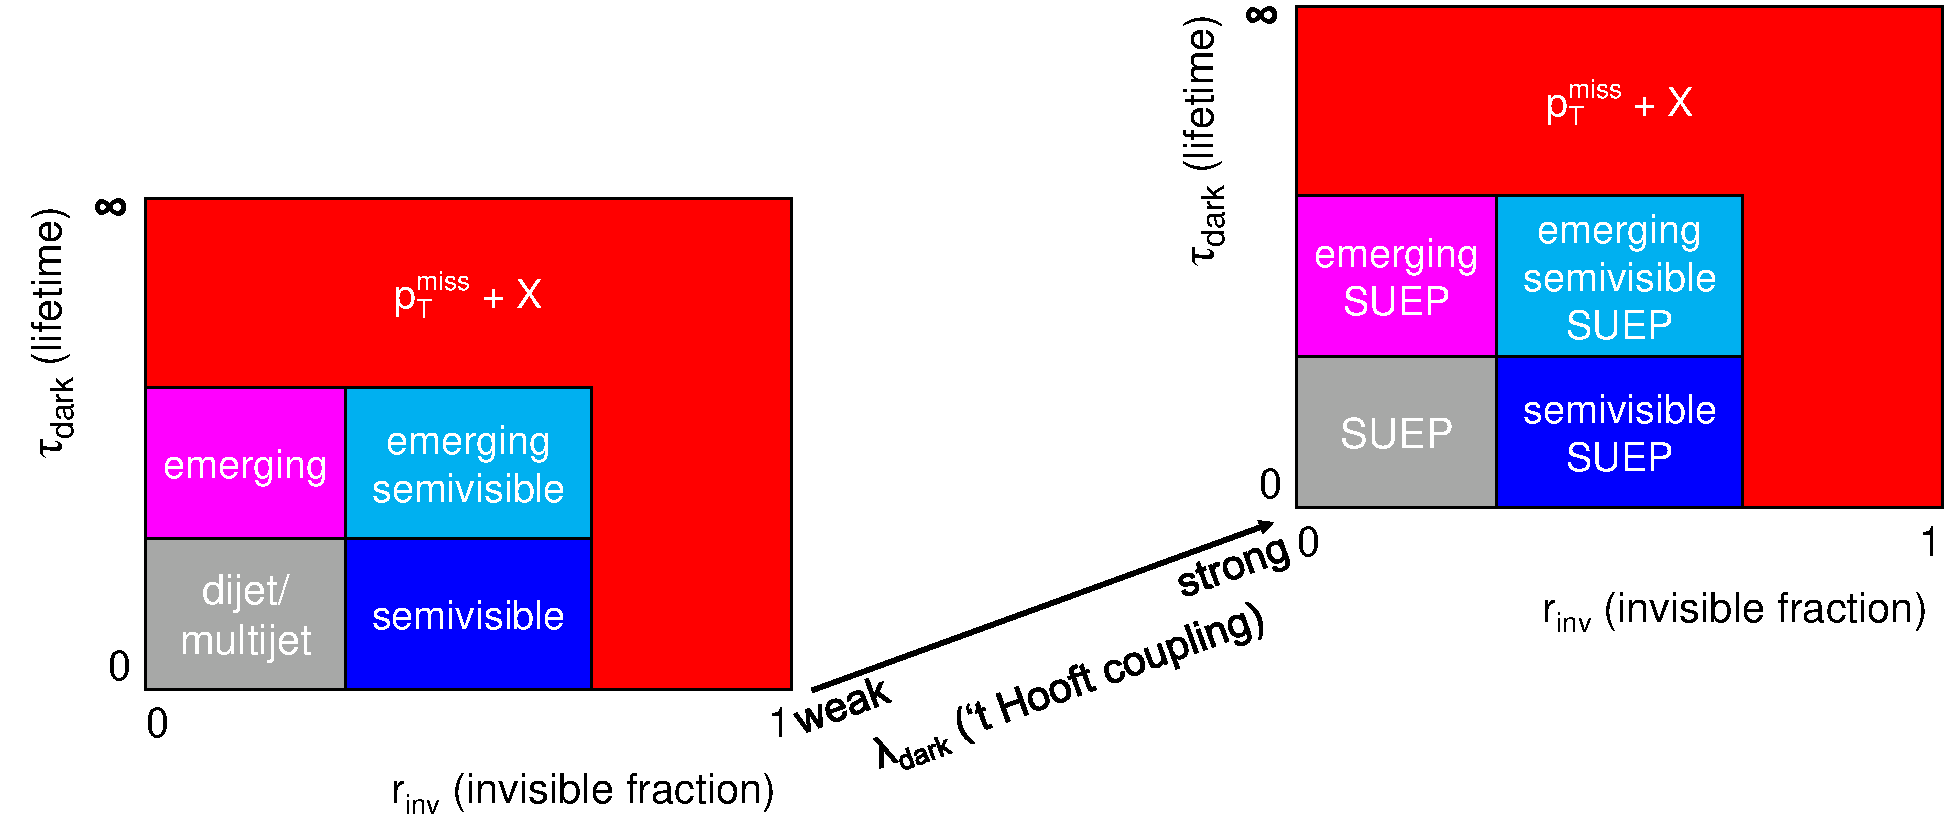
\includegraphics[width=0.95\myfigurewidth]{figures/svj_acceptance_diagram_v7.pdf}
\caption{A diagram illustrating the phenomena and search strategies with maximal acceptance for different combinations of dark QCD parameters.}
\label{fig:svjacc}
\end{figure}

However, it is not required, or even necessarily likely, that each of these phenomena should appear in isolation.
It is entirely possible that nature could produce semivisible emerging SUEPs or any other combination.
Figure~\ref{fig:svjacc} illustrates the interplay between three characteristic parameters:
the dark meson lifetime $\taudark$, the invisible fraction $\rinv$, and the 't Hooft coupling \thooft.
For large values of \rinv and \taudark, the pre-existing searches for large \met would still be the most effective.
However, for intermediate values of those parameters, a dedicated strategy might outperform any of the individual searches noted above.
The best strategies for large values of \thooft in combination with the other parameters remain an open question,
while the generation of physically realistic events at intermediate \thooft has only recently become possible~\cite{Cesarotti:2020uod}.

All of these search strategies might need adjustments for other parameters,
such as the mediator masses and couplings and the various dark sector parameters discussed in Section~\ref{subsec:models}.
The most feasible way to explore this large parameter space is using a multidimensional scan,
similar to scans of the phenomenological minimal supersymmetric standard model (pMSSM)~\cite{Djouadi:1998di}
provided by CMS for earlier datasets~\cite{Khachatryan:2016nvf,SUS-16-033-supp} and currently in preparation for Run 2 by the PI and his colleagues.
Much like the pMSSM, this scan will include many random parameter combinations, with existing constraints included to eliminate models that are already ruled out.
We will reinterpret the latest dark QCD searches from LHC Runs 2 and 3 to understand which of these combined models are effectively excluded and which are not covered.
Finding uncovered models will direct efforts to design new search strategies, including dedicated triggers, for the upcoming HL-LHC runs.
The combined models will also help to further characterize any observed signal, which would likely have intermediate values of some parameters.

Obtaining the strongest results from the dark QCD scan relies on the success of the Run 3 SVJ search.
The proposed strategy includes several new elements, any of which may not converge on the necessary timescale.
However, each new element is independent from the others, and reasonable fallback options exist to mitigate these risks:
\begin{enumerate}
\item \textit{Model building}: if a comprehensive set of new benchmarks is not available, the existing models can be used, at the cost of potentially reduced coverage of the model space.
\item \textit{Anomaly triggers}: if the anomaly trigger performance is not sufficient, the Run 2 trigger strategy can be used, at the cost of more effort to analyze multiple datasets with a less unified strategy.
\item \textit{SVJ taggers}: if the WNGAE encounters difficulties, the existing tagger architectures can be reused, at the cost of decreased tagging performance or increased model dependence. (The same applies to other AI algorithms, which can be substituted with standard techniques at the cost of increased uncertainty or decreased sensitivity.)
\end{enumerate}
At minimum, the SVJ search will benefit from the use of the larger, higher energy Run 3 dataset.
Current searches do not exclude a \PZprime of mass 6\TeV, or alternatively pair production of \Pbifun with mass 3\TeV;
the discovery significance for these models will increase by a factor of 2.0--2.4.
This is driven primarily by the 80\% higher production cross section at $\sqrt{s}=13.6\TeV$ compared to 13\TeV
and secondarily by the increase in integrated luminosity from 138\fbinv to ${\sim}$190--260\fbinv.

\section{Fast Detector Simulation}\label{sec:ml4sim}

\subsection{Background}\label{subsec:simbkg}

Full detector simulation using \GEANTfour~\cite{Agostinelli:2002hh} is highly accurate, but computationally costly:
it consumed 40\% of grid CPU usage by the major LHC experiments during Run 2~\cite{Apostolakis:2018ieg}.
This limits the number of simulated events that can be produced, directly increasing uncertainties and reducing sensitivity.
In particular, SVJ searches (Section~\ref{sec:darkqcd}) require large background samples to design optimal strategies
and large signal samples for thorough scans of all of the signal model parameters.
However, \textbf{statistical uncertainty in simulation impacts the entire collider physics program}, including measurements of the Higgs boson.

\begin{figure}[htb!]
\centering
\twofigeqh{figures/cpu_cms2022.pdf}{figures/cpu_pie_cms2022.pdf}
\caption{Left: projected CPU needs will exceed available resources for CMS in Run 3 (LHC) and Runs 4--5 (HL-LHC) without substantial R\&D.
Right: proportions of CPU usage by activity during Run 4, showing reconstruction (RECO and RECOSIM) as the largest, while simulation (SIM) remains the second-largest.
Reproduced from Ref.~\cite{CMS-NOTE-2022-008}.
}
\label{fig:cmsoffcomp}
\end{figure}

The severity of this problem will increase dramatically for the HL-LHC, which will provide an order of magnitude more data,
along with growth in per-event complexity from the associated detector upgrades.
Figure~\ref{fig:cmsoffcomp} illustrates the extreme computing challenges in the HL-LHC era.
The proportion of computing used for reconstruction increases because of superlinear scaling of key algorithms with the number of collisions per event.
Reconstruction has received substantial attention and effort to pursue algorithmic and technical improvements,
such as GPU implementations of tracking and pulse shape fitting already deployed by CMS in Run 3~\cite{Bocci:2020pmi}.
However, the challenges facing simulation have been relatively underserved;
it remains the second-largest contributor after reconstruction, so dedicated, coordinated effort is needed.
The CPU time used by the full detector simulation is expected to increase by a factor of 3 or more~\cite{Pedro:2020kbk},
because the detector upgrades introduce more complex geometries and higher precision requiring more detailed physics models.

The CMS detector simulation already benefits from numerous technical optimizations and physics-preserving approximations,
which improve its CPU efficiency by a factor of 4--6 compared to baseline \GEANTfour, as demonstrated by the PI~\cite{Pedro:2019mkq}.
The PI also led the effort to integrate a modernized CPU-based simulation engine in the CMS software (CMSSW)~\cite{Pedro:2020kbk},
which achieved a factor of 2 speedup~\cite{Amadio:2020ink}.
He now consults on the implementation of the GPU-based simulation engine Celeritas~\cite{Tognini:2022nmd} in CMS;
this project offers promising gains in simplified examples, but its performance with the full CMS geometry and physics interactions has yet to be established.
\textbf{Generative AI offers an alternative and complementary approach to achieve substantial speedups using GPUs, highlighted in the recent DOE report}~\cite{AI4SES}.

\subsection{Objectives}\label{subsec:simobj}

For a generative AI algorithm to become a broadly useful replacement for full detector simulation,
it must provide a similar level of quality while substantially increasing computational efficiency.
The PI formed and leads the CMS Machine Learning for Simulation (ML4Sim) group, and previously convened the HEP Software Foundation Detector Simulation Working Group
and the Theoretical Calculations and Simulation topical group for the Snowmass Computational Frontier~\cite{Boyle:2022cvo,Elvira:2022wyn}.
Through these roles, he is directing the field toward an emphasis on practical usability of generative AI:
the desired level of quality must be reached in order for any increase in computational speed to be meaningful.
Recently, diffusion models have come to dominate generative tasks in industry, such as the popular text-to-image generators Stable Diffusion, DALL${\cdot}$E, and Midjourney.
The PI has demonstrated that diffusion models can produce simulations of the necessary quality in public datasets~\cite{Amram:2023onf},
exceeding the performance of other approaches~\cite{Adelmann:2022ozp,Hashemi:2023rgo}.

We will apply diffusion models to simulate particle showers in the CMS calorimeters, which are the major contributor to increasing per-event simulation time at the HL-LHC~\cite{Pedro:2020kbk}.
We pursue two complementary paths for the AI algorithms (1, 2), both deployed in the same way (3):
\begin{enumerate}
\item the ``fully generative'' approach, producing showers from completely random input (Section~\ref{subsec:diffu});
\item the ``hybrid'' approach, producing showers from approximately correct input (Section~\ref{subsec:refine});
\item integrate in the experiment software using the ``inference as a service'' approach (Section~\ref{subsec:iaas}).
\end{enumerate}
We target percent-level agreement with \GEANTfour and at least a factor of 100 improvement in throughput by using GPU coprocessors.
Both are achievable given existing results, with further increases to the speed of diffusion expected as part of the project.
Any remaining discrepancies between the full and AI-based simulations will be handled by an existing, simpler form of the hybrid approach~\cite{Bein:2023ylt}.
\textbf{The readiness of the entire AI-based CMS simulation chain before the HL-LHC startup will facilitate the Run 3 capstone dark QCD scan, as well as all future Run 4 activities.}

The impact of AI-based simulation will be felt even at colliders beyond the HL-LHC.
P5 has recommended~\cite{P5:2023} an increase in R\&D toward future higher-energy colliders
to further our exploration of the universe, including the nature of dark matter.
In particular, the report highlights a muon collider as a path to 10\TeV parton center-of-mass energy, potentially at Fermilab.
\textbf{Simulation studies are one of the first critical items to understand the feasibility and design of the muon collider and its detectors.}
These simulations face an even greater challenge: the beam-induced background (BIB), from muon decays in flight, produces unprecedented particle multiplicity
such that a single event currently takes 24 hours to simulate in \GEANTfour.
A combination of the Celeritas GPU-based classical simulation engine and AI-based simulation using diffusion models will be necessary to handle the BIB at scale.
Delivering this application by the end of the grant will help ensure the success of the next generation of collider experiments.

\subsection{AI-based Simulation for CMS}

\subsubsection{Step 1: Fully Generative Simulation}\label{subsec:diffu}

Diffusion models are a type of generative AI, inspired by the physical process of diffusion.
Starting from some input data, such as images or calorimeter showers,
a training dataset is built by deterministically adding different amounts of randomness to each image.
Because the amount of randomness in each training image is known, the diffusion model can learn how to perform the addition of randomness to any data.
The objective of the model is simply a regression task, and therefore the training converges reliably.
Figure~\ref{fig:illus} shows how adding randomness repeatedly, over many iterations, produces an image that is purely random.
To generate new images, this process is reversed, starting from pure randomness to produce realistic data (``denoising'').

\begin{figure}[htb!]
\centering
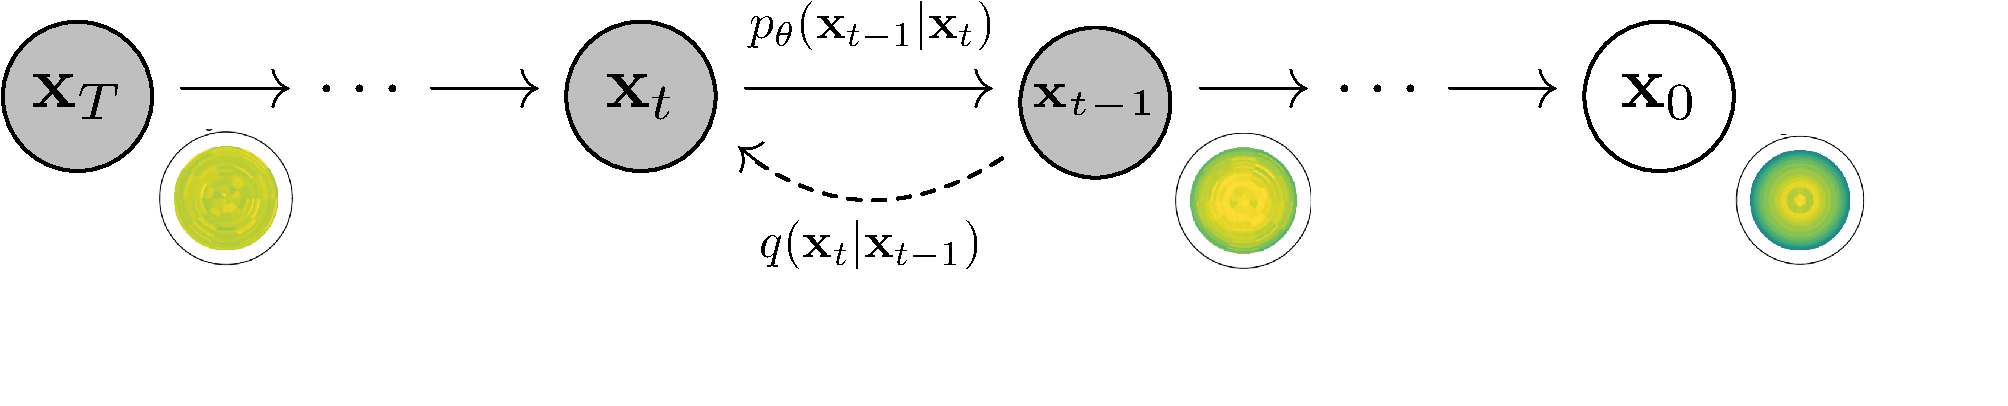
\includegraphics[width=0.95\myfigurewidth]{figures/pgm_diagram_xarrow_showers.pdf}
\caption{An illustration of the diffusion process, going from pure randomness (left) to a realistic particle shower (right) in a transverse slice of a calorimeter. Adapted from Ref.~\cite{Ho:2020}.}
\label{fig:illus}
\end{figure}

The PI and his team developed the \diffu algorithm for the \challenge,
a recent community effort to compare different AI approaches to the simulation of particle showers in calorimeters, using common datasets and metrics~\cite{CaloChallenge}.
The datasets include sampling calorimeters with varying materials and granularities and different particles including photons, pions, and electrons.
\diffu uses convolutional operations, which are computationally efficient because they share parameters and act on local data.
Several novel geometric adaptations were developed to help the convolutions handle non-rectangular and irregular calorimeter geometries.
Figure~\ref{fig:calodiffu} (left) shows results from the \challenge on the pion dataset, \textbf{clearly demonstrating the superiority of \diffu,
which is found to produce the highest quality showers for all datasets}~\cite{Krause:2023mlj}.
The algorithms are compared based on metrics including classifier scores and the Fr\'echet particle distance~\cite{Kansal:2022spb}.
This version of the algorithm is published in Ref.~\cite{Amram:2023onf};
subsequently, the quality has been improved even further, as shown in Fig.~\ref{fig:calodiffu} (right), by adding a separate module that learns the per-layer deposited energy.

\begin{figure}[htb!]
\centering
\twofigeqh{figures/ds1-pions_CE_1.pdf}{figures/FCC_ERatio_dataset2_oct11_layer_norm_Diffu.pdf}
\caption{Left: example comparison of the separation power (a $\chi^2$-like measure of the similarity between distributions~\cite{Diefenbacher:2020rna})
from the shower center of energy between AI algorithms and \GEANTfour in the community \challenge, adapted from Ref.~\cite{Krause:2023mlj}.
\diffu has the lowest values, showing that it is almost identical to \GEANTfour.
Right: The total deposited energy for the improved version of \diffu compared to \GEANTfour.}
\label{fig:calodiffu}
\end{figure}

\textbf{Here, we propose to adapt \diffu to the more complex and variable CMS geometry.}
First, we will adapt the model to the existing, simpler CMS calorimeters,
in order to deliver the necessary simulation for the dark QCD scan (Section~\ref{subsec:darkscan}).
This also serves as a useful intermediate step toward the most involved case,
the High Granularity Calorimeter (HGCal), a part of the HL-LHC detector upgrades
that will increase the number of channels by almost two orders of magnitude.
The HGCal will have both hexagonal and rectangular cells in different regions, with different material types and thicknesses.
It is also the major driver of the predicted increase in \GEANTfour simulation time~\cite{Pedro:2020kbk}.
Further optimizations of the \diffu model will be needed to handle the high dimensionality and precision requirements of this new detector.

\diffu runs 10-100 times faster than \GEANTfour by processing particles in large batches on GPUs.
While the initial version required 400 denoising iterations or ``steps'' to produce high-quality output,
the improved version requires a factor of 4--8 fewer steps, depending on the dataset, because of its intrinsically higher quality.
More recently, some of the PI's colleagues have used \diffu as a platform to test further improvements to both the training and inference~\cite{Jiang:2024ohg},
and the most promising of these have been integrated into the model~\cite{Amram:GitHub}.
Numerous other avenues to make the algorithm faster while preserving quality are under investigation~\cite{Rombach:2022,Song:2023,Mei:2023}.
These illustrate a critical advantage of diffusion models:
\textbf{because of the massive interest in these models in the broader ML community and in industry,
new methods are constantly being developed that can be easily imported for HEP use cases,}
relying on the collaborative nature of open-source software.

\textit{Risk mitigation}: if the various approaches to speed up the fully generative diffusion model do not succeed,
this will reduce the amount of simulation that can be produced,
though we still expect to exceed \GEANTfour when running in batches on GPU.
Based on existing results, the fully generative diffusion model will almost certainly produce higher quality output than existing fast simulation (FastSim) approaches in CMS~\cite{Sekmen:2016iql}.
However, if it does not, Section~\ref{subsec:refine} includes alternative approaches to improve the existing FastSim.

\subsubsection{Step 2: Hybrid Simulation}\label{subsec:refine}

\begin{wrapfigure}[21]{L}{0.5\textwidth}
\centering
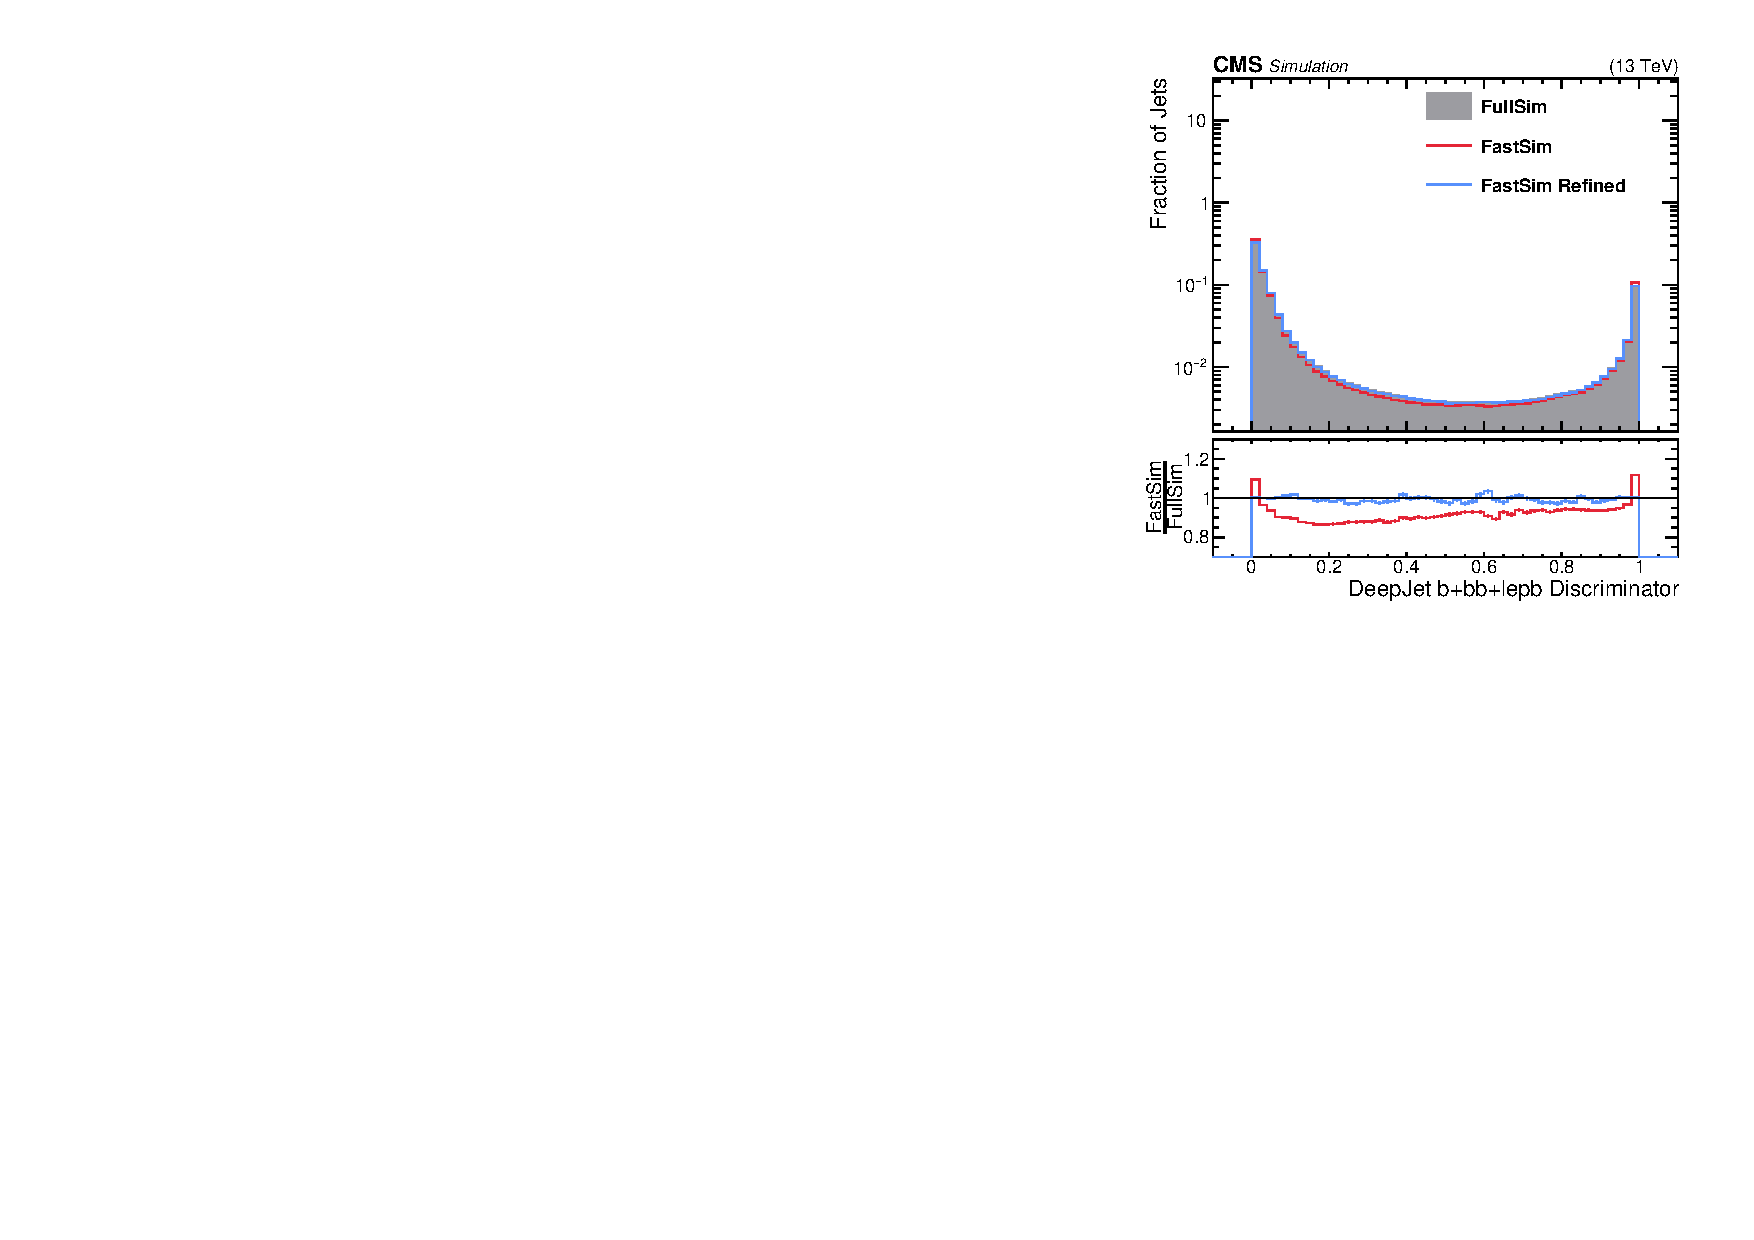
\includegraphics[width=0.46\myfigurewidth]{figures/regression_1D_20221127_DeepFlavB.pdf}
\caption{The distribution of the \DEEPJET \cPqb-jet tagging discriminator: FastSim deviates from \GEANTfour by ${\sim}10\%$, while refined FastSim has percent-level agreement with \GEANTfour.}
\label{fig:refine}
\end{wrapfigure}

Refining a low-quality simulation to obtain high-quality output was the objective of the PI's previous denoising project, which used a less sophisticated AI architecture~\cite{Banerjee:2022gkg}.
Diffusion models are much more capable, but so far the ``fully generative'' approach (producing a shower from pure randomness) has been pursued;
this is because the sampling algorithms applied during the inference steps rely on the Gaussian nature of the randomness.
The differences between FastSim and \GEANTfour will not be Gaussian, so while it is easier in principle to learn the difference between two similar distributions,
additional mathematical formalism must be derived in order to reuse the existing diffusion approach.
Ref.~\cite{Mei:2023} provides an alternative approach to achieve the same goal:
\textbf{feeding information from FastSim into the fully generative model in order to guide the diffusion to generate high-quality output in just one inference step}.

The PI and his team have also developed a complementary high-level refinement, directly targeting analysis-level variables~\cite{Bein:2023ylt}.
With promising results on \cPqb-jet tagging variables, shown in Fig.~\ref{fig:refine},
the algorithm is now being expanded to other jet-related variables and validated for use in Run 3.
The approach can be understood as a significantly more precise, correlation-preserving alternative to traditional, manually-calculated correction factors.
Given that the CMS FastSim currently only agrees with \GEANTfour to within ${\sim}10\%$,
\textbf{high-level refinement alone can substantially reduce the quality deficits in FastSim samples and the resulting uncertainties.}

The combination of diffusion and refinement will be even more powerful.
In the chain FastSim~$\to$~diffusion~$\to$~refinement, each ML algorithm solves a progressively easier problem,
because the difference with respect to the previous step is smaller.
Therefore, it can learn the solution more precisely from a given dataset size,
as well as incorporating physics at different levels: individual detector hits and reconstructed kinematic variables.
\textbf{Refinement will address any residual disagreements between FastSim-based \diffu and \GEANTfour,
resulting in a more accurate final product}, much like next-to-leading order matrix element calculations increase in accuracy by incorporating higher-order effects.

\textit{Risk mitigation}: if methods to combine the diffusion model with the existing FastSim do not succeed,
we can use the fully generative diffusion model or high-level refinement alone, at the cost of reduced computing speed or increased uncertainty, respectively.

\subsubsection{Step 3: Inference as a Service}\label{subsec:iaas}

AI algorithm inference uses a restricted set of operations, such as matrix multiplications, which can naturally be accelerated on coprocessors.
The PI is the lead developer for the Services for Optimized Network Inference on Coprocessors (SONIC) approach, which implements inference as a service.
SONIC allows seamless utilization of coprocessors in experiment software, with demonstrated inference speedups of multiple orders of magnitude,
for CMS, ATLAS, the Deep Underground Neutrino Experiment (DUNE), the Laser Interferometer Gravitational-Wave Observatory (LIGO), and analysis facilities~\cite{Duarte:2019fta,Krupa:2020bwg,Wang:2020fjr,Rankin:2020usv,Gunny:2021gne,Cai:2023ldc,CMS:2024twn,Savard:2023wwi}.
The underlying framework takes advantage of open-source tools, including the Nvidia Triton inference server~\cite{nvidia} and advances in machine learning packages.

The latest results for SONIC in CMS are shown in Fig.~\ref{fig:sonic}:
ParticleNet inference throughput can be increased up to a factor of 100 by using GPUs with the optimal backend software configuration~\cite{CMS:2024twn}.
This approach essentially eliminates the impact of AI algorithm inference on event throughput,
and the use of asynchronous, non-blocking requests~\cite{Bocci:2020olh} further eliminates the impact of latency when connecting to remote coprocessors,
at least up to a distance of hundreds of kilometers.
A single coprocessor, located anywhere, can serve tens or even hundreds of CPU processes.
SONIC has already been shown to work with GPUs, FPGAs, TPUs (tensor processing units), and IPUs (intelligence processing units).

\begin{wrapfigure}[19]{r}{0.5\textwidth}
\centering
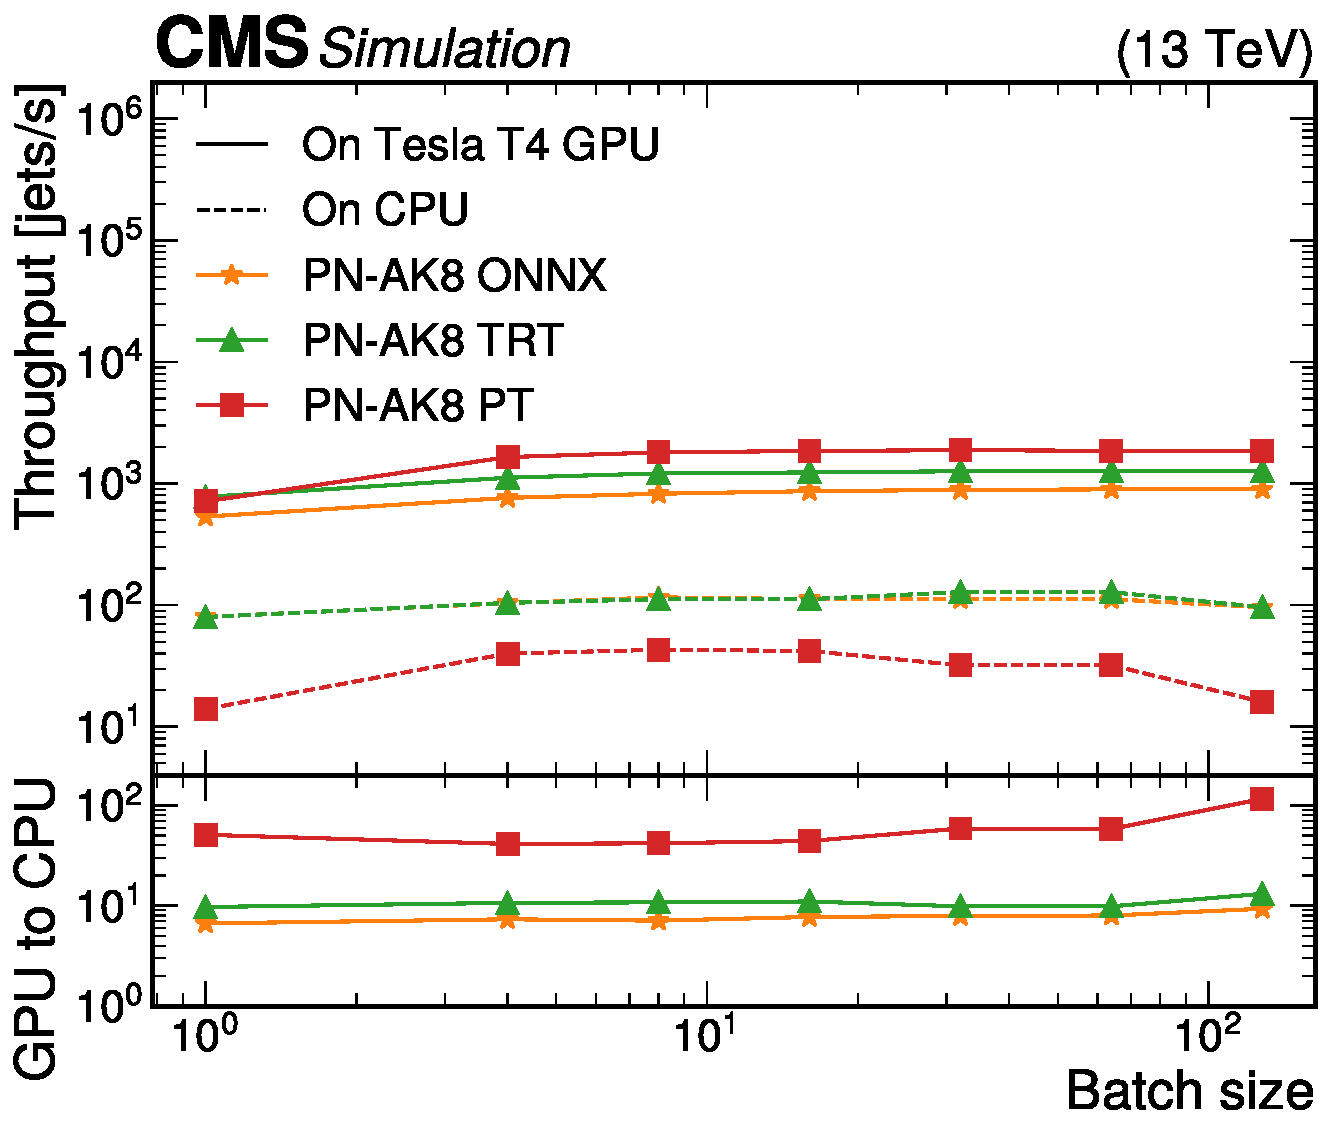
\includegraphics[width=0.49\myfigurewidth]{figures/CMS-MLG-23-001_Figure_005-b.pdf}
\caption{The inference throughput for ParticleNet on CPU and GPU, using ONNX, TensorRT, and PyTorch backends. PyTorch on GPU provides the largest throughput increase.}
\label{fig:sonic}
\end{wrapfigure}

As noted in Section~\ref{subsec:diffu}, the maximum speedup for AI-based simulation is achieved by performing inference on GPU
and generating showers for at least 100 particles simultaneously.
In order to reliably fill the GPU register memory, particles from multiple events must be processed together.
In addition, most CPUs in the Worldwide LHC Computing Grid currently are not directly connected to GPUs.
These considerations point to SONIC as the right approach to integrate AI-based simulation into experiment software frameworks.
\textbf{The PI has nearly unparalleled expertise in implementing simulation engines and inference as a service in experiment software},
through his previous roles in CMS software management and current role as lead developer of SONIC.
Deploying AI-based simulation via SONIC provides a path for efficient utilization of HPC resources and even new, unforeseen coprocessors.

\textit{Risk mitigation}: if unforeseen complications are encountered in the use of inference as a service,
directly-connected GPUs can be employed, at the cost of limiting the computing sites where simulation can be run effectively.

\textbf{The final product of this work is an AI-augmented simulation engine
that carries out rule-based algorithms on local CPUs and AI inference on remote GPUs via SONIC.}
A common implementation for diffusion model inference will be shared between the \GEANTfour and CMS FastSim interfaces to ensure consistency and minimize the maintenance burden.
Implementation in the experiment software is critical to validate the performance of either the fully generative or hybrid approach.
This requires comparisons of reconstruction-level quantities that can only be computed using the entire CMSSW processing chain.
The technologies and innovations in this part of the proposal have mostly been proven to work in other contexts, as shown above.
Viable alternatives exist to mitigate the risks from the new elements.

\subsection{Future Colliders}\label{subsec:mucoll}

If dark QCD exists but the hidden valley only couples to the SM via mediators at the 10\TeV scale, collider DM production will require a future, higher energy accelerator.
The new P5 report~\cite{P5:2023} specifically highlights a muon collider as an attractive option to reach parton center-of-mass energies of 10\TeV,
both because of its compact footprint and because of the numerous technological innovations and synergies that would be achieved in the course of constructing and operating this machine.
\textbf{While the collider itself is several decades away, the report highlights that research into its feasibility must start now.}
Simulation is a crucial component of the design process for both the detectors and the collider,
and the machine-detector interface (MDI) is particularly important for the muon collider.
The MDI must incorporate mitigations for the beam-induced background (BIB) caused by muon decays in flight as the beam circulates.
At $\sqrt{\smash[b]{s_{\Pgm\Pgm}}} = 10\TeV$, there are ${\sim}10^5$ muon decays per meter, leading to ${\sim}10^8$ photons and neutrons per bunch crossing~\cite{Black:2022cth}.

Currently, it takes 24 hours to simulate just one BIB event with \GEANTfour.
AI-based BIB simulation, therefore, would be highly impactful for muon collider, detector, and MDI design.
While \diffu is trained on single-particle events, because material interactions in \GEANTfour are modeled independently for every particle,
it may not be feasible to continue such an approach for events with $10^8$ particles.
If so, we will implement a ``grouped'' approach, in which similar particles are grouped together to train the diffusion model to generate their energy deposits together.
However, as previously noted, the output of the diffusion model must be validated by comparison to full simulation to ensure its reliability.
It is a challenging prospect for \GEANTfour even to produce a sufficient validation sample at these multiplicities.
This is an area where the new GPU-based simulation engine Celeritas offers several advantages.
The physics processes by which photons and neutrons deposit energy are limited,
with electromagnetic (EM) processes already implemented in Celeritas and neutron transport implemented in its precursor Shift~\cite{Hamilton:2018}.
The staggering multiplicity of BIB particles will ensure efficient use of GPUs for optimal throughput.
In these conditions, Celeritas may provide up to a factor 30--40 speedup compared to \GEANTfour~\cite{Tognini:2022nmd}.

After completing the previous steps in this project,
we will apply the diffusion model to simulate BIB for muon collider detector design.
The results will be validated against Celeritas simulations incorporating EM and neutron physics and the MDI geometry.
Based on existing results, we expect \diffu to provide a significant speedup even compared to Celeritas.
This combination of new approaches to simulation illustrates another facet of the synergies in the proposed muon collider program.
Further, given that BIB events also consume substantial disk space, 8--36 GB per event,
encoding this information in a diffusion model can be considered a form of compression:
the model trades disk usage for computing power by being able to generate BIB events on the fly,
requiring only $\mathcal{O}(\text{MB})$ learned weights and a source of randomness.
\textbf{This novel application of AI-based simulation will facilitate improved designs and
better projections of the physics potential of the next generation of the energy frontier.}

\section{Conclusion}\label{sec:conclusion}

This proposal puts forth a novel program to uncover the origins of dark matter
by searching for evidence of strongly coupled dark sectors or ``dark QCD''
using the Compact Muon Solenoid (CMS) experiment at the Large Hadron Collider (LHC).
The program is complementary to other ongoing efforts:
direct detection and annihilation experiments have highly suppressed sensitivity to these models.
Previous collider searches have overlooked their novel phenomenological signatures,
including semivisible jets, emerging jets, and soft unclustered energy patterns.
Expanding on the initial explorations in the LHC Run 2 dataset,
we will increase the model independence of the trigger, jet identification, and search regions,
in order to conduct a unified Run 3 search for semivisible jets covering the entire model space.
The latest unsupervised artificial intelligence (AI) techniques will be employed throughout,
even as we continue to build more thorough models of the behavior of dark QCD.
Finally, we will scan combinations of all dark QCD phenomena to identify unconstrained signatures
and design the next steps in the program for the upcoming HL-LHC.

To facilitate this program as well as many other LHC searches and measurements,
we will develop fast and accurate detector simulation using generative AI.
Using cutting-edge diffusion models and applying the latest acceleration techniques,
we will generate particle showers at least 100 times faster than CPU-based full detector simulation software.
The algorithms will be deployed on coprocessors across the computing grid using inference as a service,
the most efficient and portable approach.
In addition to enabling the dark QCD scan over the entire model space,
AI-based simulation will resolve a major computing challenge for the high luminosity LHC upgrade.
The same techniques, in combination with new GPU-based classical simulation engines,
will push forward the design of the future muon collider and its detector systems
by simulating the beam-induced background (BIB) from muon decays in flight.

The PI is uniquely suited to deliver both aspects of the proposal.
His expertise and leadership in dark QCD, AI algorithms, detector simulation, inference on coprocessors, and experiment software are widely acknowledged.
As a Fermilab scientist, he can leverage the lab's computational and theory expertise and direct the lab's facilities to ensure success.
The results will significantly advance the mission of the DOE Office of Science to search for physics beyond the standard model and to make optimal use of national computing resources.

\subsection{Timetable of Activities and Deliverables}

Table~\ref{tab:activities} summarizes the steps, contributors, and deliverables in each part of the proposal (Sections~\ref{sec:darkqcd} and~\ref{sec:ml4sim}).
Budget years (BYs) 1 and 2 correspond to the remaining years of LHC Run 3, while BY5 corresponds to the final year of the long shutdown before HL-LHC operations commence.
The last two budget years are devoted to the final, most ambitious deliverables: the dark QCD scan and future collider simulation.
The deliverables include new dark QCD models in BY2, at least one limited-author AI algorithm publication and the Run 3 semivisible jet search publication in BY3, and the full dark QCD scan publication in BY5.
On the technical side, we will deliver the AI-based simulation for CMS in BY3 and for the muon collider in BY5, with corresponding publications.

The PI and postdoctoral research associate (RA) will co-lead both the dark QCD searches and the AI-based simulation development.
Their effort will be supplemented by two AI associates (AIAs).
AIA\#1 will focus on the optimization of new AI algorithms for jet tagging, jet mass, and diffusion during BYs 2--3.
AIA\#2 will implement the AI-based diffusion in the experiment software framework using inference as a service during BYs 4--5, ensuring its scalability and smooth operation in high performance computing sites.
This distribution of personpower ensures maximal effort is available leading up to and during BY3, when several deliverables are expected.

\begin{table}[!hbtp]
\vspace{\myfigurespacing}
\begin{center}
\begin{tabular}{cccccc}
Deliverable & BY1 & BY2 & BY3 & BY4 & BY5 \\
\hline
\multicolumn{6}{c}{}\\[-\cmsTabSkip]
Dark QCD model building & \multicolumn{2}{c}{\cellcolor{blue!25} PI, RA} & & & \\
Anomaly trigger commissioning & \multicolumn{2}{c}{\cellcolor{blue!25} PI, RA} & & & \\
Jet tagger and mass variable development & \multicolumn{3}{c}{\cellcolor{blue!25} PI, RA, AIA\#1 $\ast$} & & \\
Run 3 semivisible jet search & & \multicolumn{2}{c}{\cellcolor{blue!50} PI, RA $\ast$} & & \\
Dark QCD scan & & & \multicolumn{3}{c}{\cellcolor{blue!75} PI, RA $\ast$} \\
\multicolumn{6}{c}{}\\[-\cmsTabSkip]
Generative AI development & \multicolumn{3}{c}{\cellcolor{orange!25} PI, RA, AIA\#1 $\ast$} & & \\
Hybrid simulation approach & \multicolumn{3}{c}{\cellcolor{orange!25} PI, RA, AIA\#1} & & \\
Inference as a service for simulation & & \multicolumn{3}{c}{\cellcolor{orange!50} PI, RA, AIA\#2} & \\
Future collider simulation & & & & \multicolumn{2}{c}{\cellcolor{orange!75} PI, RA $\ast$} \\
\end{tabular}
\vspace{\myfigureskip}
\caption{A summary of the activities and deliverables for the strongly coupled dark matter searches and fast detector simulation development in each budget year. The contributions of the PI, RA, and AIAs are noted. The symbol $\ast$ indicates an expected publication.}
\label{tab:activities}
\end{center}
\end{table}

\clearpage


\end{spacing}
